\chapter{程式講解}
\section{程式講解}
\begin{figure}[hbt!]
\begin{center}
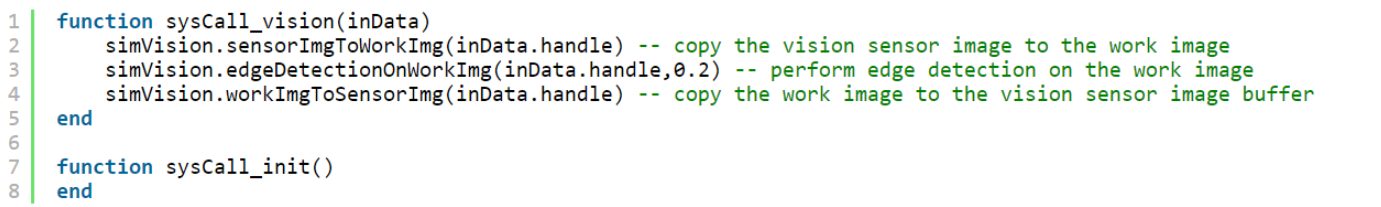
\includegraphics[width=16cm]{程式講解1}
\caption{\Large 程式講解}\label{程式講解}
\end{center}
\end{figure} 
首先這是一個Lua語言,在CoppeliaSim仿真環境中運行。該腳本定義了兩個函數:sysCallinit和sysCallvision。
\\
sysCallinit函數是仿真環境初始化時自動調用的函數,該函數目前是空的,即不執行任何操作。
\\
sysCallvision函數是CoppeliaSim的視覺模組塊(VisionModule)在每次運行時會調用的函數,該函數的作用是對視覺傳感器的圖像進行邊緣檢測(edge detection)。\\具體來說,函數中的三個函數調用分別為:
\begin{itemize}
%=----------simVision.sensorImgToWorkImg----------=%
\item simVision.sensorImgToWorkImg (圖.\ref{程式講解}):\\
將視覺傳感器的圖像複製到工作圖像中。\\
%=----------simVision.edgeDetectionOnWorkImg----------=%
\item simVision.edgeDetectionOnWorkImg (圖.\ref{程式講解}):\\
對工作圖像進行邊緣檢測,檢測閾值為0.2。\\
%=----------simVision.workImgToSensorImg----------=%
\item simVision.edgeDetectionOnWorkImg (圖.\ref{程式講解}):\\
將處理後的工作圖像複製回視覺傳感器的圖像緩衝區中。\\
其中,inData是一個包含了視覺模組塊的一些信息的table對象,例如handle(視覺傳感器的句柄)等。simVision是CoppeliaSim中提供的用於處理視覺相關任務的庫。\\
\end{itemize}
\begin{figure}[hbt!]
\begin{center}
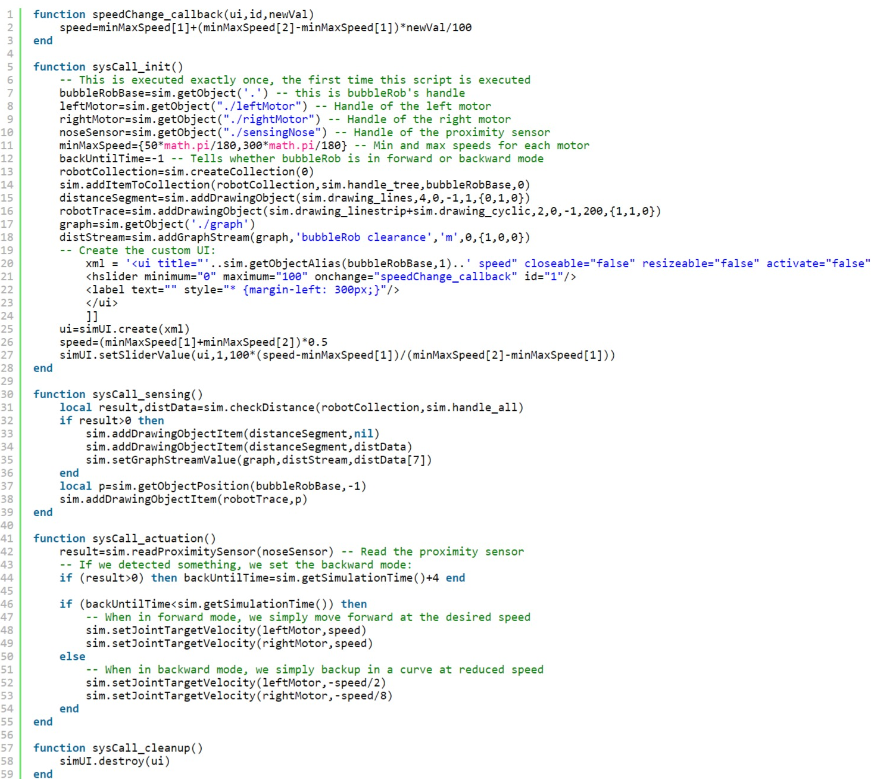
\includegraphics[width=16cm]{程式講解2}
\caption{\Large 程式講解2}\label{程式講解2}
\end{center}
\end{figure} 

如(圖.\ref{程式講解2}):
1至3行這個函數會在使用者調整了速度控制UI元素後被呼叫。它接收3個參數:ui,這是UI元素的句柄;id,這是UI元素的ID;newVal,這是UI元素的新值。函數會根據新值計算出一個速度值speed。

第5行這個函數是模擬程式的初始化函數,它只會被執行一次,當模擬程式啟動時。這個函數主要是執行一些初始化設置,例如設置模型的基礎物體、感測器和控制器,以及創建一些繪圖對象和UI元素。

第7行這行代碼會獲取模型的根物體的句柄。在這個例子中,模型的根物體是代表機器人的物體。

第8、9、10行這些行會獲取左右馬達和前方感測器的句柄。這些句柄會在後續的代碼中用於控制馬達和讀取感測器。

第11行這行會定義最小和最大速度。在這個例子中,速度是以弧度每秒為單位表示的,最小速度為50度每秒,最大速度為300度每秒。

第12行這行代碼定義了一個變數backUntilTime,用於在後續的代碼中區分機器人是向前移動還是向後移動。

第13、14行這些行代碼用於創建一個物體集合並將機器人物體添加到其中。這將使得感測器能夠檢測到機器人周圍的其他物體

第41行這個函數控制BubbleRob的行動。它首先讀取接近傳感器的數據,以檢測是否有東西在BubbleRob的前方。如果傳感器檢測到障礙物,則將backUntilTime設置為當前仿真時間加上4秒,表示BubbleRob現在處於倒車模式。否則,如果backUntilTime小於當前仿真時間,則BubbleRob處於前進模式,並且將左右馬達的目標速度設置為speed。否則,BubbleRob處於倒車模式,並且左右馬達的目標速度設置為一定的值,以實現向後行駛的效果。\\

第57行這個函數在仿真結束時被調用,以清理代碼中使用的任何資源。在這個例子中,它摧毀了UI對象,以避免內存洩漏。


\newpage
